\section{第五章
四层验证体系与Checkpoint协议}\label{ux7b2cux4e94ux7ae0-ux56dbux5c42ux9a8cux8bc1ux4f53ux7cfbux4e0echeckpointux534fux8bae}

\subsection{5.1
分层验证架构}\label{ux5206ux5c42ux9a8cux8bc1ux67b6ux6784}

\subsubsection{5.1.1 设计动机}\label{ux8bbeux8ba1ux52a8ux673a}

在任何多智能体 FPGA
设计自动化框架中，验证是保证生成代码正确性的核心环节。本框架提出的四层分级验证体系是一种通用的硬件验证方法论，适用于任何具备
Verilator 可编译 RTL 和自检 C++ Testbench
的多模块设计。传统单层验证方案（仿真通过/失败）存在以下问题：其一，语法错误只有在仿真阶段才被发现，浪费了编译资源；其二，仿真通过并不能保证边界行为的正确性；其三，子模块的独立验证通过并不意味着顶层集成的正确性。

本文提出四层分级验证体系，遵循''快速失败（fail
fast）``原则，通过逐步深入的验证策略将问题发现尽可能提前，并将验证结果与框架控制流深度集成。

\begin{figure}
\centering
\pandocbounded{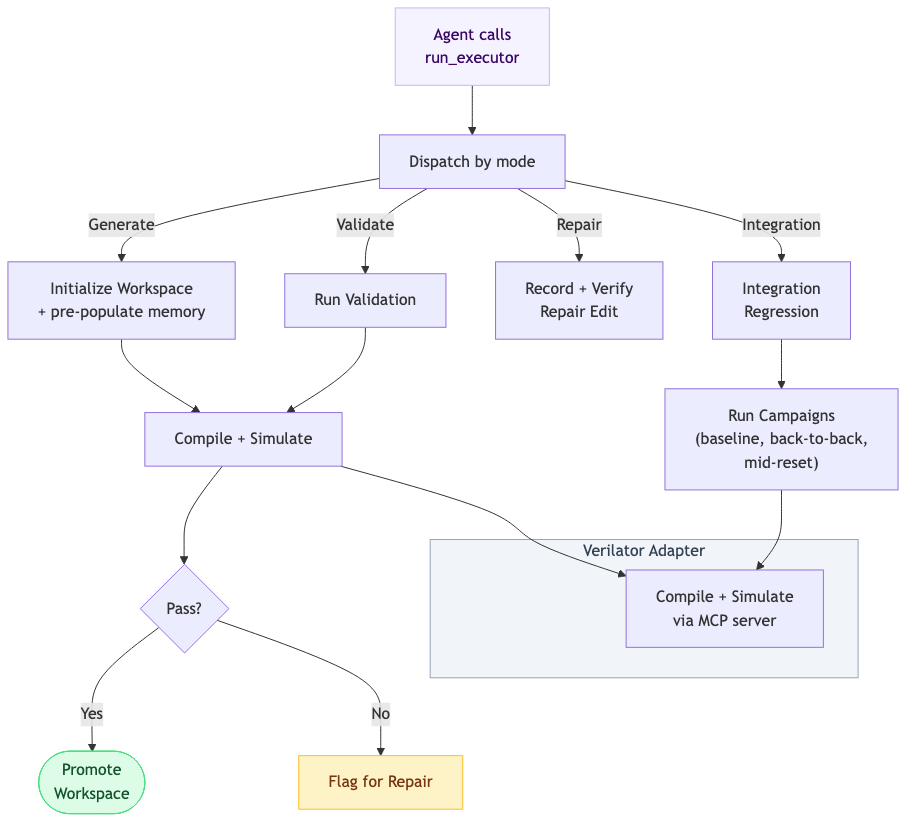
\includegraphics[keepaspectratio,alt={图5-1: 执行器调度流程}]{../fpga_flow/diagrams/08_executor_dispatch.png}}
\caption{图5-1: 执行器调度流程}
\end{figure}

四层验证体系的核心设计理念是：\textbf{时间成本与问题发现深度呈正比递增}。L0编译门控仅需秒级时间即可捕获语法级错误；L1仿真验证需要数十秒，但可验证功能正确性；L2鲁棒性测试需要分钟级时间，但能发现边界条件下的脆弱性；集成回归测试最为耗时，但能捕获模块间接口和时序问题。这一设计使系统能够在不同阶段以匹配的代价发现相应类型的问题。

\subsubsection{5.1.2
四层架构总览}\label{ux56dbux5c42ux67b6ux6784ux603bux89c8}

四层验证架构的设计不依赖于特定的硬件设计------L0 编译门控对任何 Verilog
RTL 有效，L1 Checkpoint 验证对任何实现了 Checkpoint 协议的 Testbench
有效，L2 鲁棒性测试对任何可参数化的 Testbench 有效，集成回归对任何 DAG
结构的多模块设计有效。以下以 AES-128 验证案例说明各层的具体运作。

各层验证的职责、输入输出与判定标准如下：

{[}表5-1: 各层级验证目标、输入、输出、判定标准、典型耗时{]}

\textbf{L0编译门控（L0Executor）}：接收RTL Verilog源文件和C++
Testbench，调用Verilator编译器，输出编译日志。判定标准为编译返回码为零且无错误输出。L0是最轻量的门控，能捕获未声明信号、端口宽度不匹配、语法错误、非法Verilog结构等问题。

\textbf{L1仿真验证（L1Executor）}：在L0编译成功的前提下执行仿真，通过解析\texttt{simulation.log}中的Checkpoint协议行判定功能正确性。L1采用已知向量（KAT，Known-Answer
Test），要求所有必需Checkpoint均出现且状态为PASS。

\textbf{L2鲁棒性测试（L2CampaignExecutor）}：对已通过L1的模块施加随机向量或边界向量的压力测试，验证在非KAT条件下的行为一致性。L2的判定不仅包含Checkpoint通过率，还会输出\texttt{counterexample.json}和\texttt{fragility\_summary.json}，供\texttt{L2AdaptivePlanner}用于后续Profile选择决策。

\textbf{集成回归测试（IntegrationRegressionExecutor）}：在所有模块全部PROMOTED后触发，以\texttt{IntegrationRegressionManifest}为规格驱动，对顶层模块\texttt{aes128\_encrypt\_core}执行三种Campaign（baseline、back\_to\_back、mid\_reset），验证完整系统在不同使用场景下的正确性。

\subsubsection{5.1.3
分层验证与框架控制流的集成}\label{ux5206ux5c42ux9a8cux8bc1ux4e0eux6846ux67b6ux63a7ux5236ux6d41ux7684ux96c6ux6210}

四层验证不是孤立存在的，而是与编排状态机深度集成。编排状态\texttt{MODULE\_L0}对应L0执行，\texttt{MODULE\_L1}对应L1执行，\texttt{MODULE\_L2\_OPTIONAL}对应L2鲁棒性测试，\texttt{INTEGRATION\_REGRESSION}对应集成回归测试。每层验证的判定结果直接影响工作区状态机的转移：L0失败则工作区保持REPAIRING状态，L1
Checkpoint全部通过则状态跃迁至VALIDATED，PROMOTED后触发集成回归。这一设计确保了验证结果的机器可判定性，消除了对LLM主观判断的依赖。

\begin{center}\rule{0.5\linewidth}{0.5pt}\end{center}

\subsection{5.2
Checkpoint协议设计}\label{checkpointux534fux8baeux8bbeux8ba1}

\subsubsection{5.2.1
协议格式规范}\label{ux534fux8baeux683cux5f0fux89c4ux8303}

Checkpoint 协议的格式设计是完全通用的------任何硬件设计的 Testbench
均可通过调用 \texttt{emit\_checkpoint()} 发射自定义的 Checkpoint
标记，框架的 \texttt{CheckpointParser}
无需修改即可解析。协议的通用性使得框架支持新设计时无需更改验证基础设施，只需定义新的
Checkpoint 名称集合。

Checkpoint协议是本框架验证体系的核心通信机制，定义了Testbench与框架之间的结构化结果汇报接口。协议格式为：

\begin{verbatim}
CHECKPOINT|<name>|PASS|<detail>
\end{verbatim}

其中： - \texttt{CHECKPOINT} 为固定前缀，作为日志行过滤的识别标记 -
\texttt{\textless{}name\textgreater{}}
为Checkpoint名称，与\texttt{pass\_criteria.l1.coverage\_checkpoints}中定义的名称精确对应
- \texttt{PASS} 为当前唯一合法的状态值，表示该检查点已验证通过 -
\texttt{\textless{}detail\textgreater{}}
为人类可读的补充说明，不参与机器判定逻辑

该协议通过\texttt{aes\_tb\_common.hpp}中的\texttt{emit\_checkpoint()}函数在C++
Testbench端发射：

\begin{Shaded}
\begin{Highlighting}[]
\KeywordTok{inline} \DataTypeTok{void}\NormalTok{ emit\_checkpoint}\OperatorTok{(}
    \AttributeTok{const} \BuiltInTok{std::}\NormalTok{string}\OperatorTok{\&}\NormalTok{ checkpoint}\OperatorTok{,}
    \AttributeTok{const} \BuiltInTok{std::}\NormalTok{string}\OperatorTok{\&}\NormalTok{ detail}
\OperatorTok{)} \OperatorTok{\{}
    \BuiltInTok{std::}\NormalTok{cout }\OperatorTok{\textless{}\textless{}} \StringTok{"CHECKPOINT|"} \OperatorTok{\textless{}\textless{}}\NormalTok{ checkpoint }\OperatorTok{\textless{}\textless{}} \StringTok{"|PASS|"} \OperatorTok{\textless{}\textless{}}\NormalTok{ detail }\OperatorTok{\textless{}\textless{}} \BuiltInTok{std::}\NormalTok{endl}\OperatorTok{;}
\OperatorTok{\}}
\end{Highlighting}
\end{Shaded}

（\texttt{fpga\_flow/tb/aes\_tb\_common.hpp:603-608}）

这一设计实现了Testbench端的极简接入：Testbench开发者只需在正确性验证通过后调用\texttt{emit\_checkpoint("CHK\_XXX",\ "描述")}一行代码，无需了解协议解析细节。

\subsubsection{5.2.2
设计决策分析}\label{ux8bbeux8ba1ux51b3ux7b56ux5206ux6790}

选择简单文本协议而非结构化输出（如JSON）的决策基于以下考量：

\textbf{对日志噪声的鲁棒性}：Verilator仿真过程中会产生大量警告、调试输出和波形信息。文本协议通过逐行扫描和前缀匹配实现解析，不受日志噪声干扰；而JSON格式需要完整解析仿真输出流，对格式错误极为敏感。

\textbf{Testbench端实现简单}：\texttt{emit\_checkpoint()}是单行调用，Testbench开发者和LLM
Agent均能可靠地生成该调用，不会因JSON转义、嵌套结构等问题引入格式错误。

\textbf{框架端解析简单}：\texttt{CheckpointParser}（\texttt{fpga\_flow/executors.py:71-90}）的实现仅需30行代码，通过\texttt{CHECKPOINT\_PREFIX\ =\ \textquotesingle{}CHECKPOINT\textbar{}\textquotesingle{}}前缀过滤和\texttt{split(\textquotesingle{}\textbar{}\textquotesingle{},\ 3)}分割即可完成解析，维护成本极低。

与AutoGen方案的对比：该方案使用Vivado
xsim仿真，验证结果依赖波形图（.vcd）的人工判读，无法实现机器自动判定。本文的Checkpoint协议使验证结果完全机器可判定，且与文件系统通信机制（Batch
Gate回调）无缝集成。

\subsubsection{5.2.3
CheckpointParser解析逻辑}\label{checkpointparserux89e3ux6790ux903bux8f91}

框架端的\texttt{CheckpointParser}类（\texttt{fpga\_flow/executors.py:71-90}）负责从\texttt{simulation.log}文件中提取Checkpoint信息，构建\texttt{name→status\textbar{}detail}字典：

\begin{Shaded}
\begin{Highlighting}[]
\KeywordTok{class}\NormalTok{ CheckpointParser:}
    \KeywordTok{def}\NormalTok{ parse\_text(}\VariableTok{self}\NormalTok{, text: }\BuiltInTok{str}\NormalTok{) }\OperatorTok{{-}\textgreater{}} \BuiltInTok{dict}\NormalTok{[}\BuiltInTok{str}\NormalTok{, }\BuiltInTok{str}\NormalTok{]:}
\NormalTok{        summary: }\BuiltInTok{dict}\NormalTok{[}\BuiltInTok{str}\NormalTok{, }\BuiltInTok{str}\NormalTok{] }\OperatorTok{=}\NormalTok{ \{\}}
        \ControlFlowTok{for}\NormalTok{ raw\_line }\KeywordTok{in}\NormalTok{ text.splitlines():}
\NormalTok{            line }\OperatorTok{=}\NormalTok{ raw\_line.strip()}
            \ControlFlowTok{if} \KeywordTok{not}\NormalTok{ line.startswith(CHECKPOINT\_PREFIX):}
                \ControlFlowTok{continue}
\NormalTok{            parts }\OperatorTok{=}\NormalTok{ line.split(}\StringTok{\textquotesingle{}|\textquotesingle{}}\NormalTok{, }\DecValTok{3}\NormalTok{)}
            \ControlFlowTok{if} \BuiltInTok{len}\NormalTok{(parts) }\OperatorTok{\textless{}} \DecValTok{4}\NormalTok{:}
                \ControlFlowTok{continue}
\NormalTok{            \_, name, status, detail }\OperatorTok{=}\NormalTok{ parts}
\NormalTok{            summary[name] }\OperatorTok{=} \SpecialStringTok{f\textquotesingle{}}\SpecialCharTok{\{}\NormalTok{status}\SpecialCharTok{\}}\SpecialStringTok{|}\SpecialCharTok{\{}\NormalTok{detail}\SpecialCharTok{\}}\SpecialStringTok{\textquotesingle{}}
        \ControlFlowTok{return}\NormalTok{ summary}
\end{Highlighting}
\end{Shaded}

解析器扫描\texttt{simulation.log}全文，对每一行检查是否以\texttt{CHECKPOINT\textbar{}}开头，然后以\texttt{\textbar{}}为分隔符切分（最多3次，保留detail中可能存在的\texttt{\textbar{}}字符），构建名称到状态字符串的映射。

\subsubsection{5.2.4
Checkpoint汇总与判定}\label{checkpointux6c47ux603bux4e0eux5224ux5b9a}

\texttt{summarize\_required\_checkpoints()}函数（\texttt{fpga\_flow/executor\_contracts.py:329-353}）接收解析后的Checkpoint字典和required\_checkpoints元组，输出三类分类结果：

\begin{itemize}
\tightlist
\item
  \textbf{missing}：未在仿真日志中出现的必需Checkpoint（Testbench未执行到该路径）
\item
  \textbf{failed}：出现但状态字段不为\texttt{PASS}的Checkpoint
\item
  \textbf{passed}：出现且状态为\texttt{PASS}的Checkpoint
\end{itemize}

只有当\texttt{missing}和\texttt{failed}均为空时，验证才判定为通过。这一逻辑同时捕获了''Testbench未运行到验证点''和''Testbench运行到验证点但判定失败''两种失败模式。

\begin{figure}
\centering
\pandocbounded{
\includegraphics[keepaspectratio,alt={图5-2: 批次执行循环}]{../fpga_flow/diagrams/03_batch_execution_loop.png}}
\caption{图5-2: 批次执行循环}
\end{figure}

\subsubsection{5.2.5
各模块Checkpoint一览}\label{ux5404ux6a21ux5757checkpointux4e00ux89c8}

以下 AES-128 验证案例的 9 个 Checkpoint 展示了 Checkpoint
协议在具体设计中的实例化方式。对于其他硬件设计（如 SHA-256 哈希模块或
FIFO 控制器），可按照相同的协议定义不同的 Checkpoint 集合。

{[}表5-2: 各模块Checkpoint一览表{]}

{\def\LTcaptype{none} % do not increment counter
\begin{longtable}[]{@{}
  >{\raggedright\arraybackslash}p{(\linewidth - 4\tabcolsep) * \real{0.2069}}
  >{\raggedright\arraybackslash}p{(\linewidth - 4\tabcolsep) * \real{0.4828}}
  >{\raggedright\arraybackslash}p{(\linewidth - 4\tabcolsep) * \real{0.3103}}@{}}
\toprule\noalign{}
\begin{minipage}[b]{\linewidth}\raggedright
模块
\end{minipage} & \begin{minipage}[b]{\linewidth}\raggedright
Checkpoint名称
\end{minipage} & \begin{minipage}[b]{\linewidth}\raggedright
验证内容
\end{minipage} \\
\midrule\noalign{}
\endhead
\bottomrule\noalign{}
\endlastfoot
aes\_sbox & CHK\_SBOX\_MATCH & S-box查找表输出与已知向量匹配 \\
aes\_key\_schedule\_128 & CHK\_ROUNDKEY\_MATCH &
11轮密钥扩展输出与标准参考值匹配 \\
aes\_round\_transform & CHK\_ROUND\_STATE\_MATCH &
单轮SubBytes+ShiftRows+MixColumns+AddRoundKey输出匹配 \\
aes128\_encrypt\_core & CHK\_RESET\_CLEAR & 复位后所有状态寄存器清零 \\
aes128\_encrypt\_core & CHK\_START\_ACCEPTED &
start信号在IDLE状态被正确采样 \\
aes128\_encrypt\_core & CHK\_BUSY\_ASSERTED &
加密启动后busy信号在首个时钟上升沿置位 \\
aes128\_encrypt\_core & CHK\_DONE\_PULSE &
done信号为单周期脉冲（仅持续1个时钟） \\
aes128\_encrypt\_core & CHK\_CIPHERTEXT\_MATCH &
11周期后输出密文与NIST标准向量精确匹配 \\
aes128\_encrypt\_core & CHK\_BUSY\_DEASSERTED &
done脉冲后busy信号随即去断言 \\
\end{longtable}
}

\texttt{aes128\_encrypt\_core}模块包含6个Checkpoint，覆盖了完整的FSM行为验证路径：从复位清零、握手协议、busy信号时序、延迟精度到密文正确性，构成了对11周期迭代微架构的全面行为规约。

\begin{center}\rule{0.5\linewidth}{0.5pt}\end{center}

\subsection{5.3 L2鲁棒性测试}\label{l2ux9c81ux68d2ux6027ux6d4bux8bd5}

\subsubsection{5.3.1 设计动机}\label{ux8bbeux8ba1ux52a8ux673a-1}

L1验证使用已知向量（KAT），这些向量来自NIST
FIPS-197标准，数量有限且确定性强。KAT通过并不能证明模块在随机输入、边界输入、重复模式输入等条件下行为正确。L2鲁棒性测试的目标是在L1的功能正确性验证之上，进一步探测模块的边界脆弱性。

\subsubsection{5.3.2 L2 Profile体系}\label{l2-profileux4f53ux7cfb}

L2测试通过Profile机制对测试强度进行分级控制：

\begin{itemize}
\tightlist
\item
  \textbf{rand\_small}（种子1001）：少量随机向量（默认8个case），快速探测随机条件下的基本正确性
\item
  \textbf{rand\_medium}（种子2001）：中等数量随机向量，深度随机测试
\item
  \textbf{back\_to\_back}（种子3001）：连续加密场景，无空闲间隔，验证FSM状态清理正确性（仅顶层模块适用）
\item
  \textbf{mid\_reset}（种子4001）：加密过程中断言reset，验证复位恢复行为（仅顶层模块适用）
\end{itemize}

Profile的种子固定（\texttt{\_CAMPAIGN\_PROFILE\_SEEDS}字典，\texttt{fpga\_flow/executors.py:206-211}），保证测试结果的完全可复现性。

\subsubsection{5.3.3
随机数生成与可复现性}\label{ux968fux673aux6570ux751fux6210ux4e0eux53efux590dux73b0ux6027}

随机块生成使用xorshift算法，C++实现在\texttt{aes\_tb\_common.hpp:488-501}，Python实现在\texttt{\_BaseExecutor}类中（\texttt{fpga\_flow/executors.py:219-234}）。两端实现保持严格一致，使Python生成的oracle密文（用于端到端验证）与C++
Testbench生成的随机向量完全对应。

C++端\texttt{random\_block()}函数：

\begin{Shaded}
\begin{Highlighting}[]
\KeywordTok{inline}\NormalTok{ Block random\_block}\OperatorTok{(}\DataTypeTok{uint64\_t}\OperatorTok{\&}\NormalTok{ state}\OperatorTok{)} \OperatorTok{\{}
\NormalTok{    Block out}\OperatorTok{\{\};}
    \ControlFlowTok{for} \OperatorTok{(}\BuiltInTok{std::}\NormalTok{size\_t i }\OperatorTok{=} \DecValTok{0}\OperatorTok{;}\NormalTok{ i }\OperatorTok{\textless{}} \DecValTok{16}\OperatorTok{;} \OperatorTok{++}\NormalTok{i}\OperatorTok{)} \OperatorTok{\{}
\NormalTok{        out}\OperatorTok{[}\NormalTok{i}\OperatorTok{]} \OperatorTok{=} \KeywordTok{static\_cast}\OperatorTok{\textless{}}\DataTypeTok{uint8\_t}\OperatorTok{\textgreater{}(}\NormalTok{next\_rng}\OperatorTok{(}\NormalTok{state}\OperatorTok{)} \OperatorTok{\textgreater{}\textgreater{}} \DecValTok{56}\OperatorTok{);}
    \OperatorTok{\}}
    \ControlFlowTok{return}\NormalTok{ out}\OperatorTok{;}
\OperatorTok{\}}
\end{Highlighting}
\end{Shaded}

其中\texttt{next\_rng()}为xorshift64变体（state \^{}= state
\textless\textless{} 13; state \^{}= state \textgreater\textgreater{} 7;
state \^{}= state \textless\textless{}
17），每次取64位状态的最高字节作为随机字节输出。固定seed与确定性RNG的组合确保了L2测试的完全可复现性：任意时刻以相同seed执行相同profile，必然得到相同的测试向量序列。

\subsubsection{5.3.4
顶层模块的Oracle生成机制}\label{ux9876ux5c42ux6a21ux5757ux7684oracleux751fux6210ux673aux5236}

对于\texttt{aes128\_encrypt\_core}（顶层模块），L2测试采用额外的端到端正确性验证机制。框架在仿真前调用\texttt{\_write\_campaign\_oracle\_file()}（\texttt{fpga\_flow/executors.py:239-291}），使用OpenSSL的\texttt{aes-128-ecb}命令行接口生成每个随机测试向量对应的标准密文，写入oracle文件：

\begin{verbatim}
label=rand_small_case_0|key=<32位hex>|plaintext=<32位hex>|ciphertext=<32位hex>
\end{verbatim}

Testbench读取oracle文件中的密文进行比对，实现了以OpenSSL为参考实现的端到端验证。这一设计的优势在于：oracle生成完全独立于被测模块，避免了''用自身验证自身''的循环逻辑。

\subsubsection{5.3.5
L2AdaptivePlanner自适应策略}\label{l2adaptiveplannerux81eaux9002ux5e94ux7b56ux7565}

\texttt{L2AdaptivePlanner}（\texttt{fpga\_flow/synthesis.py:930-976}）根据历史脆弱性记录自适应选择L2
Profile：

\begin{itemize}
\tightlist
\item
  若模块无历史记录，选择第一个Profile（rand\_small）
\item
  若上一次Profile测试失败，选择列表中的下一个Profile（更严格的测试）
\item
  若上一次Profile测试通过，保持当前Profile
\end{itemize}

这一机制实现了测试强度与历史脆弱性的自适应匹配，避免了对所有模块施加同等力度的测试造成的资源浪费。

\begin{figure}
\centering
\pandocbounded{
\includegraphics[keepaspectratio,alt={图5-3: 错误恢复流程}]{../fpga_flow/diagrams/13_error_recovery.png}}
\caption{图5-3: 错误恢复流程}
\end{figure}

\subsubsection{5.3.6
L2测试输出物}\label{l2ux6d4bux8bd5ux8f93ux51faux7269}

L2执行完成后输出两个关键文件：

\textbf{\texttt{counterexample.json}}：记录失败向量详情，包含profile、vecfile、cases、seed、checkpoint\_summary、missing\_checkpoints、failed\_checkpoints等字段，供框架和Agent分析失败原因。

\textbf{\texttt{fragility\_summary.json}}：记录脆弱性统计指标，包含observed\_checkpoints（实际出现的Checkpoint）、checkpoint\_count等信息，供\texttt{L2AdaptivePlanner}用于下一轮Profile决策。

\begin{center}\rule{0.5\linewidth}{0.5pt}\end{center}

\subsection{5.4
集成回归测试}\label{ux96c6ux6210ux56deux5f52ux6d4bux8bd5}

集成回归测试的三种 Campaign
模式（baseline、back\_to\_back、mid\_reset）是面向时序状态机硬件设计的通用测试策略，适用于任何包含
FSM 的多模块设计。

\subsubsection{5.4.1
触发条件与规格定义}\label{ux89e6ux53d1ux6761ux4ef6ux4e0eux89c4ux683cux5b9aux4e49}

集成回归测试的触发条件是：AES-128全系统的所有4个模块（aes\_sbox、aes\_key\_schedule\_128、aes\_round\_transform、aes128\_encrypt\_core）全部达到PROMOTED状态，且\texttt{IntegrationReadinessResolver}确认所有依赖已满足。

集成测试规格通过\texttt{IntegrationRegressionManifest}（\texttt{fpga\_flow/artifacts.py:270-294}）定义，采用Pydantic模型并强制\texttt{extra=\textquotesingle{}forbid\textquotesingle{}}，包含：

\begin{itemize}
\tightlist
\item
  \texttt{top\_module}：集成测试的顶层模块（aes128\_encrypt\_core）
\item
  \texttt{rtl\_files}：全部4个模块的RTL文件列表（含依赖关系顺序）
\item
  \texttt{tb\_file}：顶层模块的C++ Testbench
\item
  \texttt{required\_modules}：必需模块列表，与rtl\_files的stem顺序严格一致（由\texttt{model\_validator}验证）
\item
  \texttt{regression\_checkpoints}：需要在所有Campaign中通过的Checkpoint集合
\item
  \texttt{latency\_target\_cycles}：11周期延迟目标
\item
  \texttt{back\_to\_back\_required}：是否需要执行back\_to\_back Campaign
\item
  \texttt{mid\_reset\_scenarios}：mid\_reset Campaign的场景列表
\item
  \texttt{interface\_freeze\_hash}：接口冻结标识（\texttt{aes-128-block\_handshake-iterative\_10\_round-autonomous-v1}）
\end{itemize}

\texttt{synthesize\_integration\_manifest()}函数（\texttt{fpga\_flow/synthesis.py:612-658}）在框架初始化阶段从SpecIR和PlanDAG自动生成IntegrationRegressionManifest，无需人工配置。

\subsubsection{5.4.2
三种Campaign规格}\label{ux4e09ux79cdcampaignux89c4ux683c}

{[}表5-3: 三种集成Campaign规格表{]}

\textbf{baseline Campaign}：使用NIST
FIPS-197标准向量执行端到端加密正确性验证。验证目标是确认顶层模块在标准测试条件下的功能完全正确。包含全部6个aes128\_encrypt\_core
Checkpoint：CHK\_RESET\_CLEAR、CHK\_START\_ACCEPTED、CHK\_BUSY\_ASSERTED、CHK\_DONE\_PULSE、CHK\_CIPHERTEXT\_MATCH、CHK\_BUSY\_DEASSERTED。

\textbf{back\_to\_back
Campaign}：连续发起多次加密请求，两次加密之间无空闲间隔（前一次done脉冲后立即送入新的start信号）。验证目标是FSM在连续工作模式下不存在状态残留：BUSY信号在done后正确去断言，IDLE状态正确恢复，下次start能被正常采样。通过\texttt{plusargs:\ \{profile:\ \textquotesingle{}back\_to\_back\textquotesingle{}\}}传递给Testbench。

\textbf{mid\_reset
Campaign}：在加密进行到第5轮（约中间位置）时断言reset信号，验证FSM能够从任意中间状态正确复位，之后能够接受新的加密请求并产生正确密文。通过\texttt{plusargs:\ \{profile:\ \textquotesingle{}mid\_reset\textquotesingle{}\}}传递给Testbench。

集成测试捕获的典型缺陷类型包括：子模块接口时序错位（如busy信号延迟一个周期）、FSM状态寄存器复位不完全（如round计数器在reset后未清零）、back\_to\_back场景下的状态污染（如前次加密的key未清除影响后次加密）。这些缺陷在子模块独立L1验证中无法被发现，只有在系统级集成测试中才会暴露。

\subsubsection{5.4.3
集成测试执行机制}\label{ux96c6ux6210ux6d4bux8bd5ux6267ux884cux673aux5236}

\texttt{IntegrationRegressionExecutor}（\texttt{fpga\_flow/executors.py:552-693}）按以下流程执行集成回归：

\begin{enumerate}
\def\labelenumi{\arabic{enumi}.}
\tightlist
\item
  调用\texttt{resolve\_integration\_regression\_inputs()}解析manifest，验证rtl\_files顺序与required\_modules一致，验证vector\_set文件存在
\item
  执行一次编译（将全部4个模块的RTL和顶层TB一同编译为可执行模型）
\item
  依次执行baseline、back\_to\_back（如\texttt{back\_to\_back\_required}为True）、mid\_reset（如\texttt{mid\_reset\_scenarios}非空）三种Campaign
\item
  每种Campaign独立调用\texttt{simulate()}，使用独立的output\_dir，解析独立的simulation.log
\item
  使用\texttt{summarize\_required\_checkpoints()}对每种Campaign的Checkpoint进行汇总，生成aggregate\_missing和aggregate\_failed
\item
  当aggregate\_missing和aggregate\_failed均为空时，写入status:
  'passed'的\texttt{integration\_regression\_result.json}
\end{enumerate}

\begin{figure}
\centering
\pandocbounded{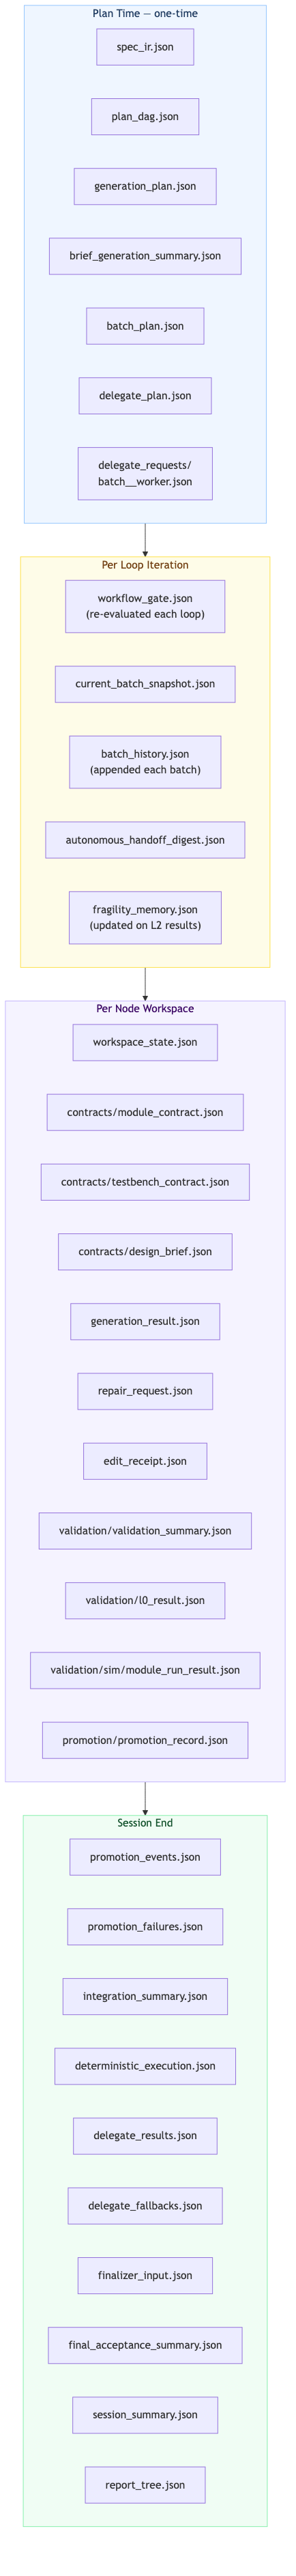
\includegraphics[keepaspectratio,alt={图5-4: JSON构件生命周期}]{../fpga_flow/diagrams/12_json_artifact_lifecycle.png}}
\caption{图5-4: JSON构件生命周期}
\end{figure}

\subsubsection{5.4.4
集成测试与子模块验证的层次关系}\label{ux96c6ux6210ux6d4bux8bd5ux4e0eux5b50ux6a21ux5757ux9a8cux8bc1ux7684ux5c42ux6b21ux5173ux7cfb}

集成回归测试在四层验证体系中处于顶层，与子模块L0/L1/L2验证形成层次关系：子模块验证关注局部行为正确性，集成验证关注系统级行为正确性和模块间交互。

本框架的设计原则是：每个模块在进入集成测试前必须经过独立的L0+L1验证（可选L2），PROMOTED状态是集成测试的前提条件。这一''先分后合''的验证策略减少了集成测试阶段的调试负担，提高了系统整体的验证效率。

四层验证体系的完整执行路径为：

\begin{verbatim}
L0编译门控 → L1仿真+Checkpoint → (L2鲁棒性测试) → 所有模块PROMOTED → 集成回归测试 → DONE
\end{verbatim}

每一层都是下一层的前提，每一层的验证结果都直接驱动框架控制流的状态转移，形成了一套机器自动判定、无需人工干预的完整验证体系。
